
\documentclass[a4paper]{tufte-handout}
%%%%%%%%%%%%%%
%  Packages  %
%%%%%%%%%%%%%%
% \usepackage{lab_notes} 
\usepackage{pgfplots}
\usepackage{tikz}
\usepackage{hyperref}
\usepackage{minted}
\usepackage[utf8]{inputenc}
\usepackage[T1]{fontenc}
\usepackage{amsmath}
\usepackage{booktabs}
\usepackage[inline]{enumitem}
\usepackage{array}
\usepackage{multicol}
\usetikzlibrary{matrix}
\usepackage{algorithmic}
\definecolor{lightBlue}{RGB}{148,176,188}
\definecolor{sexyRed}{RGB}{175,30,45}
\definecolor{sexyBlack}{RGB}{52,52,52}
\hypersetup{
    pdffitwindow=false,            % window fit to page
    pdfstartview={Fit},            % fits width of page to window
    pdftitle={Lab notes 2014},     % document title
    pdfauthor={Your Name},         % author name
    pdfsubject={},                 % document topic(s)
    pdfnewwindow=true,             % links in new window
    colorlinks=true,               % coloured links, not boxed
    linkcolor=DarkScarletRed,      % colour of internal links
    citecolor=DarkChameleon,       % colour of links to bibliography
    filecolor=DarkPlum,            % colour of file links
    urlcolor=DarkSkyBlue           % colour of external links
}


%%%%%%%%%%%%%%%
%  meta data  %
%%%%%%%%%%%%%%%
\title{Intro to Image Understanding}
\newcommand{\institution}{Self Employment}
\date{\today}

\begin{document}
\maketitle

\begin{enumerate}
%{{{Own 2D filter
\item Write your own code for computing convolution of the 2d (grayscale) image
  and a 2D filter. Make the output matrix be the same size as the input
  image.\footnote{Be cereful to correctly deal with th border of the image-
    the easiest way to do this is to "zero-pad" the image prior to
  convolution.}
  
\end{enumerate}

\begin{center}
  \begin{minted}[fontsize=\scriptsize,frame=lines]{python}

def conv_fast(image, kernel):
  """
  Function for 2D convolution using numpy
  """
    Hi, Wi = image.shape
    Hk, Wk = kernel.shape
    out = np.zeros((Hi, Wi))

    #flipping the kerne in x axis
    kernel = np.flip(kernel,axis=0);

    #padding the image
    padded= zero_pad(image, Hk//2, Wk//2)

    #loop on element
    for i in range(Hi):
        for j in range(Wi):
            out[i,j]=np.sum(padded[i:i+Hk,j:j +Wk]* kernel)

    return out
  \end{minted}
\end{center}
%}}} end Own 2D filter
%{{{Extending color images
\begin{itemize}
  \item  Extend this code to handle \emph{RGB} images. \footnote{To avoid touching
    the 1 channel convolution, we will write a wrapper to handle both
    situations.}
\end{itemize}
\begin{center}
  \begin{minted}[fontsize=\scriptsize,frame=lines]{python}

def conv_fast(image, kernel):

def conv(Img, kernel):
  """
  Generalized version to compute convolution
  with Img and kernel. The iage could be 3 channel 
  """

  #getting the number of dimensions
  if Img.ndim == 2:
    #gray scale image
    return conv_fast(image, kernel)
  else:
    #filtering in each channel
    F = np.zeros_like(Img):
    
    #loop over each channel
    for c in range(2):
      F[:,:,c] = conv_fast(Img[:,:,c])
    return F
  \end{minted}
\end{center}
%}}} end Extending color images
%{{{Composition of Convolution
\begin{itemize}
\item You convolve your image $I$ with a \emph{2d} kernel
  $K_1 =\begin{pmatrix} a & b\\c & d\end{pmatrix}$, then take the output and convolve
  it with $K_2 = \begin{pmatrix}e & f \\ g & h\end{pmatrix}$.\\[4pt]

  It is possible to get the same result with a single convolution?\\

Yes theoretically, convolution product is \textbf{associative}. Hence 

\begin{equation}
  (I * K_1) * K_2 = I * (K_1*K_2)
\end{equation}
  

The kernel $K_3 =K_1 * K_2$ has a dimension $(3,3)$ and its given
by\footnote{Convolution of the images $(n_1,m_2)$ and $(n_2,m_2)$ has a size
  of:\\

$(n_1 + n_2 - 1, m_1 + m_2 -1)$.}

\begin{equation}
  K_3 = \begin{pmatrix}
    dc & ac + db & ad \\
    bc + de & ac + bd + ec + fd & bd + df\\
    be & ae + fd & cf\\
  \end{pmatrix}
\end{equation}
\end{itemize}
%}}} end Composition of Convolution
%{{{Own Gaussian filter
\begin{itemize}
\item Write your own function that create an isotropic Gaussian filter with
  $\sigma$ and an input parameter.

First we create a function to create the \textbf{Gaussian kernel} with standard
deviation $\sigma$.
\end{itemize}

\begin{center}

 
%{{{ Gaussian kernel
  \begin{minted}[fontsize=\scriptsize,frame=lines]{python}
def Gaussian_kernel_2d(sigma=1):
    """
    Gaussian kernel in the 2d case
    """
    #number of points after 3 stds
    N = int(3*sigma)

    #distances
    d = np.r_[ np.arange(-N,0), np.arange(0,N+1)]
    n = len(d)

    #diff in X
    X = np.tile(d, (n,1))
    Y = X.transpose()

    cst = 1/(2 * np.pi * sigma**2)

    Z = cst * np.exp(-(X**2 + Y**2)/(2*sigma**2))

    return Z/ np.sum(Z)

  \end{minted}
\end{center}
%}}}

And now, we simply use the convolution function with the Gaussian kernel

%{{{ Gaussian Filter
  \begin{minted}[fontsize=\scriptsize,frame=lines]{python}
def Gaussian_filter(Img, sigma=1):
    """
    Gaussian filter with given sigma
    """

    #getting the kernel
    kernel = Gaussian_kernel_2d(sigma)


    #computing the convolution
    return conv_fast(Img, kernel)
  \end{minted}
%}}}
%}}} end Own Gaussian filter
%{{{Convolving with Waldo
  \begin{itemize}
\item Use a Gaussian filter and produce the results of convolving a Gaussian
  filter with the \emph{Waldo} image.
\end{itemize}

  \begin{marginfigure}
    \centering
    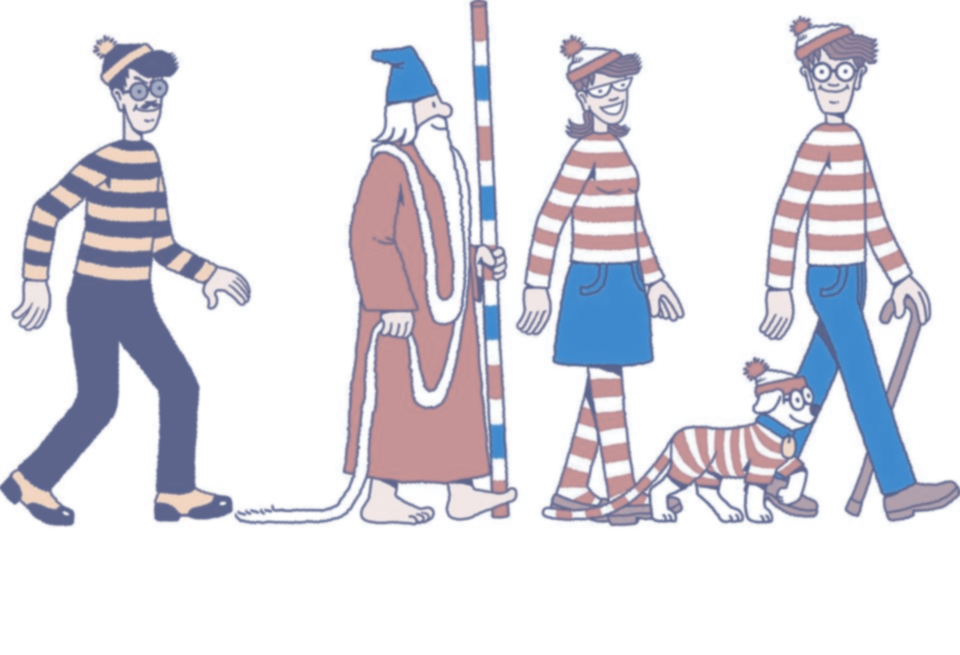
\includegraphics[width=5cm, height=3cm]{./waldo_gauss_c.png}
    \caption{Results of the convolution with $\sigma=1$}
  \end{marginfigure}
%}}} end Convolving with Waldo
%{{{Separability for partial derivative
Is the vertical derivative, $\dfrac{\partial G(x,y)}{\partial y}$ of a Gaussian filter a separable filter?

Yes, as the original filter is seprable.

\begin{eqnarray}
  G(x,y) &  = & \dfrac{1}{2\pi \sigma^2}\; e^{-\dfrac{x^2 + y^2}{2\sigma^2}}\\
         &  = & \big(\dfrac{1}{\sqrt{2\pi} \sigma}\;e^{\dfrac{-x^2}{2\sigma^2}}\big)
\big(\dfrac{1}{\sqrt{2\pi} \sigma}\;e^{\dfrac{-y^2}{2\sigma^2}}\big)\\
        &   = & G_x G_y\\
  \dfrac{\partial G(x,y)}{\partial y} & =  & G_x \partial_y(G_y) 
\end{eqnarray}
%}}} end Separability for partial derivative
%{{{Complexity for separable
\begin{itemize}
  \item What is the number of operations for performing a 2D convolution?
  \item What is the number of operations in the case of \emph{separable} filter?
\end{itemize}

The number of operation\footnote{assuming a simple convolution not convolution
by fourier transform}, the number of quadratic in term of the images size and
kernel size

\begin{equation}
  C(\text{Conv}) = \mathcal{O}(NMkl)
\end{equation}

For a \textbf{separable filter} the complexity is :

\begin{equation}
  C(\text{Conv}_{sep}  = \mathcal{O}(NMk) + \mathcal{O}(NMl)
\end{equation}
%}}} end Complexity for separable
%{{{Gadient Magnitude
\begin{itemize}
  \item Compute the \textbf{gradient magnitude} for the \texttt{waldo} image and
    the \texttt{template}?
\begin{marginfigure}
  \centering
  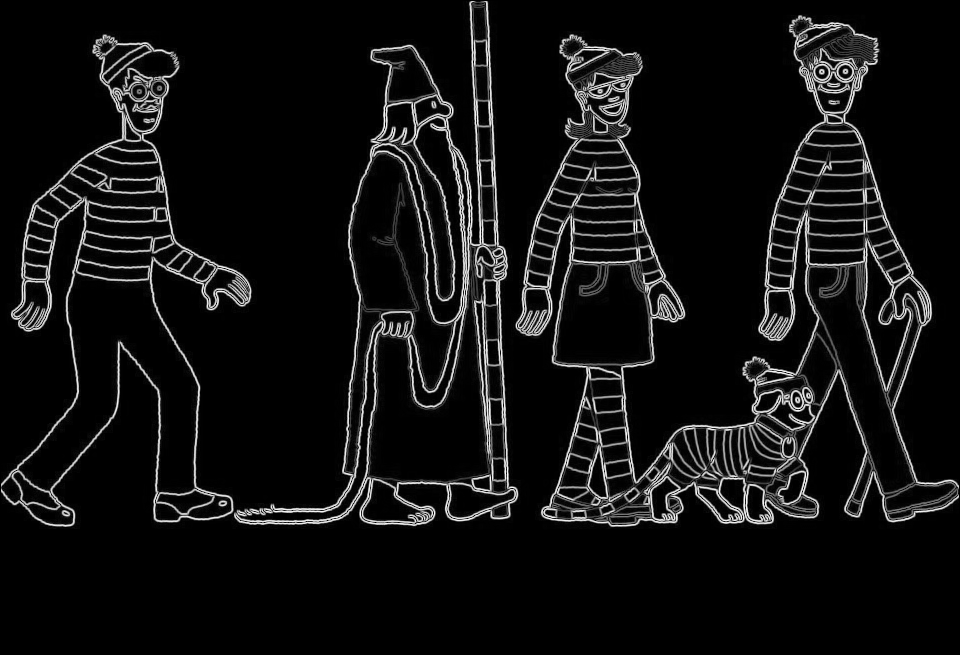
\includegraphics[width=5cm, height=3cm]{./waldo_ESM.png}
  \caption{Waldo Edge Strenght map}
\end{marginfigure}

\begin{marginfigure}
  \centering
  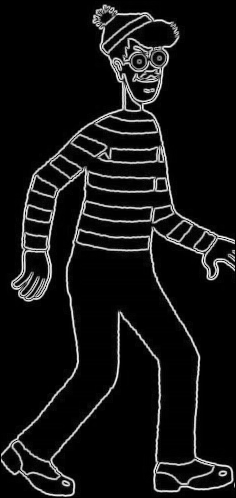
\includegraphics[width=5cm, height=3cm]{./template_ESM.png}
  \caption{Template edge strenght map}
\end{marginfigure}
\end{itemize}
%}}} end Gadient Magnitude

%{{{Localization by edge map strenght
\begin{itemize}
  \item Write a function to localize  the template ( \texttt{template.png})
    using the Edge Strenght Map?
\end{itemize}

As a first step we write the \emph{Normalized Cross Corelation} routine to
perform the correlation with the normalized patchs.

\begin{center}
  \begin{minted}[frame=lines, fontsize=\scriptsize]{python}

    """
    Function to performe the corss corelation to find waldo
    """

    #IMG
    Img = imread("./waldo_ESM.png")
    Img = rescale(Img, 0.5)
    #template
    patch = imread("./template_ESM.png")

    #position
    x, y = np.unravel(np.argmax(scors), scores.shape)

    scores = np.abs(correlate(Img, patch))
    # plt.imshow(scores, cmap = plt.cm.gray)
    imsave("./matching.png", scores)

  \end{minted}
\end{center}


\begin{marginfigure}
  \centering
  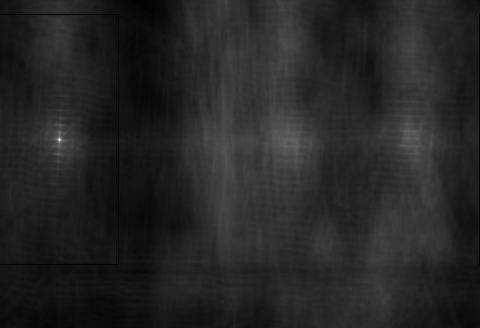
\includegraphics[width=5cm, height=3cm]{./matching.png}
\end{marginfigure}
%}}} end Localization by edge map strenght

\end{document}
